\section{Discussion and Open Problems}
\vspace{10pt}

The results presented suggest a deep connection between symbolic modular potentials, prime-induced Hamiltonians, and the non-trivial zeros of the Riemann zeta function. While numerical evidence and structural alignment support the framework, several critical open questions remain before a definitive spectral proof can be claimed.

\begin{enumerate}
  \item \textbf{Infinite-Dimensional Limit of \( \hat{H} \):}  
  Formalize the limit \( N \to \infty \) of the finite Hermitian matrix \( \hat{H}_N \to \hat{H}_\infty \) within a well-defined Hilbert space \( \mathcal{H}_P \), and establish essential self-adjointness and compactness conditions.
  
  \item \textbf{Spectral Trace Regularization:}  
  Rigorously define \( \zeta_{\hat{H}}(s) = \operatorname{Tr}(\hat{H}^{-s}) \), including convergence domain, analytic continuation, and functional equation, possibly via heat kernel or zeta-function regularization techniques.

  \item \textbf{Analytic Connection to \( \zeta(s) \):}  
  Prove that \( \zeta_{\hat{H}}(s) \equiv \zeta(s) \) either via direct spectral correspondence \( \lambda_n = \gamma_n \) or by establishing that the completed operator zeta function \( \xi_{\hat{H}}(s) \) shares the same zeros and functional symmetry.

  \item \textbf{Symbolic Resonance Dynamics:}  
  Develop a formal theory of symbolic resonance convergence, including proof that \( \Theta_k(p) \to 1 \) in the infinite prime limit under modular-resonant flow. This may imply convergence of \( \hat{H}_\infty \) toward an eigenbasis aligned with the zeta zeros.

  \item \textbf{Uniqueness and Universality of \( \hat{H}_\infty \):}  
  Determine whether the constructed operator is unique (up to unitary equivalence) or belongs to a broader class of spectral generators for \( \zeta(s) \), and explore implications for universality of prime-based quantum systems.

  \item \textbf{Experimental Realizability:}  
  Propose a physical or computational system that can simulate \( \hat{H}_\infty \) and measure its spectral properties, potentially linking this framework to quantum computing, entropy-based resonators, or symbolic AI systems.
  \item \textbf{Modular Generalization:}
  Investigate the framework's dependence on the specific modulus \(m=12\). Test other moduli (e.g., \(m=6, 10, 24\)) to determine if the observed spectral alignment is robust or an artifact of this particular choice. Analyze how the structure of prime-rich residue classes for different \(m\) influences the results.
  % TODO: Perform numerical tests for different moduli m and analyze results.
\end{enumerate}

\begin{figure}[h]
\centering
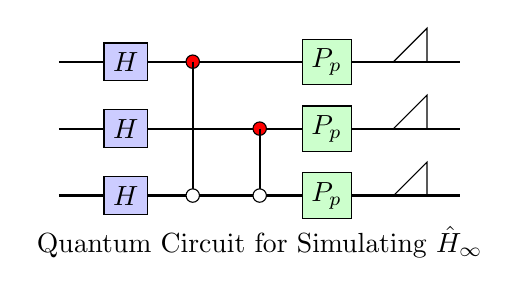
\begin{tikzpicture}[scale=0.85]
    % Draw quantum computing circuit diagram
    \draw[thick] (0,0) -- (6,0);
    \draw[thick] (0,1) -- (6,1);
    \draw[thick] (0,2) -- (6,2);
    
    % Draw quantum gates
    \node[draw, fill=blue!20] at (1,0) {$H$};
    \node[draw, fill=blue!20] at (1,1) {$H$};
    \node[draw, fill=blue!20] at (1,2) {$H$};
    
    % Draw controlled operations
    \draw[fill=red] (2,2) circle (0.1);
    \draw[thick] (2,2) -- (2,0);
    \draw[fill=white] (2,0) circle (0.1);
    
    \draw[fill=red] (3,1) circle (0.1);
    \draw[thick] (3,1) -- (3,0);
    \draw[fill=white] (3,0) circle (0.1);
    
    \node[draw, fill=green!20] at (4,0) {$P_p$};
    \node[draw, fill=green!20] at (4,1) {$P_p$};
    \node[draw, fill=green!20] at (4,2) {$P_p$};
    
    % Add measurement symbols
    \draw (5,0) -- (5.5,0.5) -- (5.5,0) -- (5,0);
    \draw (5,1) -- (5.5,1.5) -- (5.5,1) -- (5,1);
    \draw (5,2) -- (5.5,2.5) -- (5.5,2) -- (5,2);
    
    % Add caption
    \node at (3,-0.7) {Quantum Circuit for Simulating $\hat{H}_\infty$};
\end{tikzpicture}
\caption{A conceptual quantum circuit that could be used to simulate the spectral properties of the operator $\hat{H}_\infty$, with prime-indexed quantum gates.}
\label{fig:quantum_circuit}
\end{figure}

Solving these problems would not only complete a constructive spectral proof of the Riemann Hypothesis but also illuminate new physical and computational manifestations of prime-based quantum structure.